% Encoding: utf-8
% Project documentation.
\documentclass[a4paper,10pt]{article}

% Packages
\usepackage[utf8]{inputenc}
\usepackage{czech}
\usepackage{url}
\usepackage{graphicx}
% \usepackage{unicode-math}

% Omicron fake (because I am not using proper pdflatex compiler)
\newcommand{\Omicron}{O}

\title{Paralelní a distribuované algoritmy \\Projekt č. 2 \-- Implementace Enumeration Sort}
\author{Daniel Dušek, xdusek21@stud.fit.vutbr.cz}

% Some pretty neat values, probably invented by Petr Zemek (https://github.com/s3rvac)
\setlength{\hoffset}{-1.5cm}
\setlength{\voffset}{-1.5cm}
\setlength{\textheight}{23.0cm}
\setlength{\textwidth}{15.2cm}

\begin{document}

    \maketitle

	\section{Rozbor a analýza algoritmu}
	\label{sec:rozbor}
    	\par Algoritmus \textit{Enumeration Sort} realizovaný za pomoci lineárního pole \textit{n} procesorů se společnou sběrnicí, je paralelním řadícím algoritmem. Každý z procesorů obsahuje  4 registry X, Y, Z a C, jejichž účel je popsán níže v této sekci. 

    	\hspace{0.2cm}

    	\textbf{Princip paralelního algoritmu Enumeration Sort}

    	\begin{enumerate}
    		\item Všechny C registry se nastaví na hodnotu 1.
    		\item Následující činnosti se opakují 2n krát 1 $\leq $ k $\leq$ 2n:
    			\begin{itemize}
    				\item{Je-li na vstupu prvek $x_i$, vloží se sběrnicí do registru $X_i$ a lineárním spojením do $Y_1$.}
    				\item{Každý procesor, jehož registry $X$ a $Y$ nejsou prázdné provede jejich porovnání a je-li $X>Y$\footnote{V implementované verzi algoritmu je navíc zavedena podmínka $X \geq Y$, dle článku \textit{The Parallel Enumeration Sorting Scheme for VLSI od autorů Hiroto Yasuura, Naofumi Takagaki, Shuzu Yajima}, kterou je zajištěna funkčnost i při výskytu více shodných čísel} inkrementuje svůj registr $C$}
    				\item{Obsah všech registrů $Y$ se posune doprava.}
    				\item{Je-li vstup vyčerpán ($k>n$), procesor $P_{k-n}$ pošle sběrnicí obsah svého registru $X$ procesoru $P_{Ck-n}$ a ten jej uloží do svého registru $Z$ }
    			\end{itemize}
    		\item V následujících \textit{n} cyklech procesory posouvají obsah svých registrů $Z$ doprava na procesor $P_n$, který produkuje seřazenou posloupnost.
    	\end{enumerate}

    	\par Z výše popsaného principu algoritmu plyne, že jeho asymptotická složitost lze vyjádřit rovnicí $\Omicron \left(1\right) + \Omicron \left(2*n\right) + \Omicron \left(n\right)$. Proměnná \textit{n} zde reprezentuje počet řazených hodnot. Členy rovnice v~takovém pořadí, v~jakém jsou uvedeny, odpovídají krokům výše uvedeného algoritmu, tedy \textit{počáteční nastavení registrů}, \textit{distribuce a porovnávání hodnot} a nakonec \textit{produkce hodnot na kořenovém procesoru}. Potom tedy platí, že čas potřebný k řešení úlohy (v krocích) $t\left(n\right) = \Omicron\left(n\right)$. 

    	\par Dále víme, že cena paralelního řešení je vyjádřena vztahem $c\left(n\right) = p\left(n\right) * t\left(n\right)$, kde $p\left(n\right)$ je počet procesorů, z toho vyvodíme, že cena tohoto paralelního algoritmu je rovna $\Omicron\left(n^2\right)$ a tedy není optimální.


    	\par Registr $X$ slouží k uchování hodnoty přiřazené procesoru na začátku před řazením. Skrze registr $Y$ prochází hodnoty, které jsou v průběhu řazení porovnávány a posouvány směrem doprava. Během těchto porovnávání je inkrementován registr $C$, jehož hodnota určuje počet prvků menších než je hodnota registru $X$. Do registru $Z$ se po konci první fáze kroku algoritmu umístí hodnota odpovídajícího procesoru $X$ tak, aby posuvy ke kořenovému procesoru došlo k vygenerování seřazené posloupnosti.

	\section{Implementace}
	\label{sec:implementace}
    	\par Jako implementační jazyk byl zvolen jazyk C++ s využitím knihovny Open MPI. 
    	\par Kód programu je rozdělen do dvou význačných proudů \-- větve pro řídící, tzv. kořenový, proces, jehož běh simuluje běh řídícího procesoru a větve, kterou se vydávají procesy \uv{pracovníků}, které simulují \uv{pracovnické} procesory.

    	\par Kořenový proces čte sekvenčně ze souboru \textit{numbers} posloupnost náhodných čísel v rozsahu 0-255 a posílá je postupně skrze sběrnici podřízeným procesům. Po přečtení každého čísla jej také pošle lineárním spojením do registru $Y_1$. Během načítání hodnot a jejich distribuce navíc kořenový proces postupně vypisuje načtená čísla v takovém pořadí, v jakém je získal. Následně již kořenový proces jen vyčkává než mu ostatní, podřízené procesy, začnou hlásit seřazené hodnoty posloupnosti. Tyto hodnoty převezme a vypíše na standardní výstup.
    	
    	\par Pracující procesy přebírají hodnoty od kořenového procesu a provádí řazení hodnot tak, jak je dáno principem algoritmu. 
    	
    	\par Z konkrétních funkcí knihovny Open MPI je používáno pro meziprocesorovou komunikaci zejména funkcí \texttt{MPI\_Recv()} a \texttt{MPI\_Send()} a na jednom místě programu navíc funkce \texttt{MPI\_Barrier()}, jako synchronizačního prostředku, který nepropustí žádný proces dál, dokud všechny ostatní procesy z~komunikační skupiny nedorazily do stejného bodu. Bariéra je použita před začátkem posílání hodnot do kořenového procesu, aby bylo se 100\% jistotou zajištěno, že každý proces odesílá seřazenou hodnotu.

	\section{Měření a experimenty}
	\label{sec:mereni}
		\par Implementace algoritmu byla podrobena měření, kdy byl měřen čas potřebný k seřazení různého počtu hodnot. Toto měření probíhalo na autorově pracovní stanici, kdy v průběhu celého měření bylo dbáno na stejné konstatní zatížení prostředí, aby docházelo k minimálnímu počtu chyb způsobených prostředím. Pro každou získanou hodnotu bylo provedeno 30 měření. Z naměřených 30 hodnot byly odstraněny očividné chyby měření a ponechané hodnoty byly zprůměrovány. 

		\par Stejné experimenty byly provedeny i na školním testovacím server \textit{Merlin} a výsledný časový trend byl takřka shodný s trendem naměřeným na autorově stanici. Časově se hodnoty ovšem lišily \-- na školním serveru byly řádově nižší (toto si autor vysvětluje jako rozdíl v HW konfiguraci).

		\par Pro měření doby běhu skriptu bylo využito funkce \texttt{MPI\_Wtime()} volané na vhodných místech v~kódu \-- a sice před začátkem řadícího algoritmu a po jeho konci, zevnitř těla kořenového procesu. Umístění funkcí do kořenového procesu je dostatečné a oprávněné, neb moment, kdy kořenový procesor zná správné pořadí řazených prvků je zároveň i moment, kdy algoritmus doběhl. Protože kořenový proces čeká na odpověď od všech podřazených procesů, je opravdu zachycená celá doba běhu algoritmu. Dvě získané hodnoty od sebe potom byly odečteny a tím byla získána opravdová doba běhu algoritmu. 
    	
    	\par V Tabulce~\ref{tab:1} je vyobrazena závislost času potřebného k seřazení hodnot, na počtu těchto hodnot (\textit{Pozn. tabulka je zde uvedena pouze pro úplnost}). Hodnoty v tabulce jsou právě výše zmíněné, naměřené a zprůměrované výsledky. Na základě těchto hodnot byl také vytvořen graf zobrazující časovou závilost na počtu prvků.


	\begin{table}[th]
		\centering
		\caption{\textbf{Závislost času potřebného k seřazení na počtu řazených prvků}}
		\label{my-label}
		\begin{tabular}{l||ccccccccc}
		 \hline \hline
		 počet prvků & 2 & 3 & 5 & 8 & 10 & 13 & 15 & 18 \\
		 \hline
		 čas [s]     & 0.0031 & 0.0045 & 0.0090 & 0.0138 & 0.0152 & 0.0123 & 0.0237 & 0.0337  \\
		   &    &    &    &    &   \\
		   &    &    &    &    &   \\
		 \hline
		 počet prvků  & 20 & 23 & 25 & 28 & 30 \\
		 \hline
		 čas [s]  & 0.0337 & 0.0480 & 0.0539 & 0.0772 & 0.0594 \\
		  \hline
		 \label{tab:1}
		\end{tabular}
	\end{table}


	\begin{figure}[th]
	\centering
	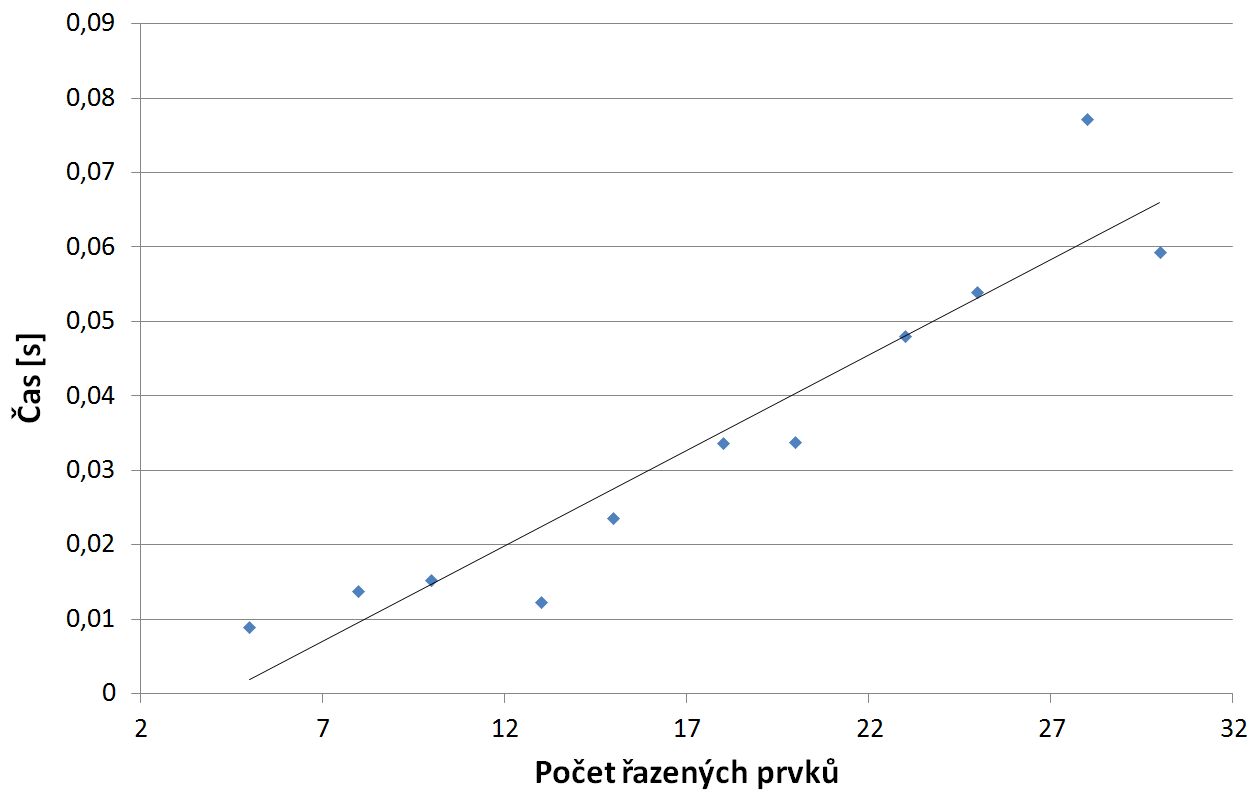
\includegraphics[width=0.85\textwidth]{graph.PNG}
	\label{fig:graph}
	\caption{Graf závislosti času potřebného k seřazení prvků na jejich počtu}
	\end{figure}	


	\section{Komunikační protokol procesů}
	\label{sec:comprot}
    	\par Meziprocesorová komunikace je simulována pomocí funkcí poskytovaných MPI knihovnou \texttt{MPI\_Recv()} a \texttt{MPI\_Send()}. Pomocí těchto funkcí je simulována jak komunikace po sběrnici, tak lineární propojení procesorů. Knihovna MPI navíc poskytuje další užitečné funkce jako je \texttt{MPI\_BCast} či \texttt{MPI\_Gather}, které by mohly být využity při dalších možných optimalizacích implementovaného algoritmu (popsáno níže). Sekvenční diagram meziprocesové komunikace je zachycen na obrázku~2.

		\begin{figure}[h!]
    	\centering
    	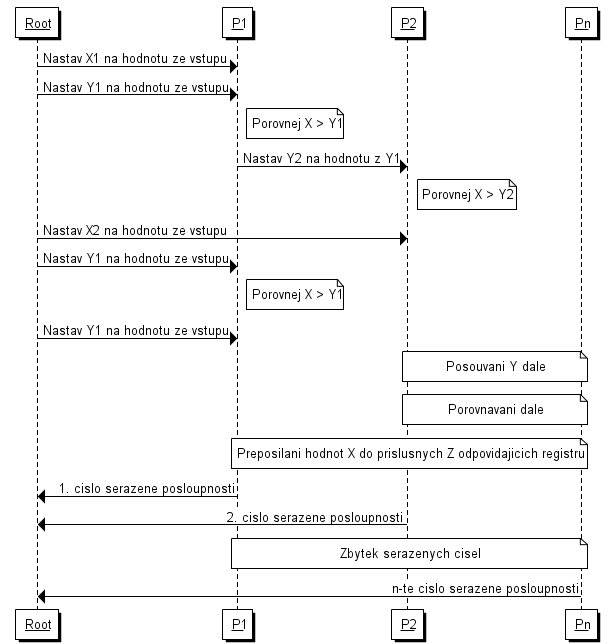
\includegraphics[width=0.75\textwidth]{process_communication.png}
    	\label{fig:sequence-diagram}
    	\caption{Sekvenční diagram meziprocesové komunikace.}
    	\end{figure}

    \section{Navrhované modifikace algoritmu}
    \label{sec:proposedmodifications}
    \par Při modifikované implementaci algoritmu \textit{enumeration sort} by bylo možné využít funkcí knihovny MPI, a to  \texttt{MPI\_Scatter()} a \texttt{MPI\_Bcast()} pro efektivnější distribuci čísel k podřazeným procesorům. Dále by pak navíc bylo při předávání výsledků možné zrychlit předávání hodnot zpět ke kořenovému procesoru využitím funkce \texttt{MPI\_Gather()}. Odhadované snížení složitosti při použití těchto funkcí by mohlo být až o $\Omicron\left(n\right) + \Omicron\left(n\right)$.
    \par Autor by rád odůvodnil překročení rozsahu 3 stran právě touto sekcí, kterou na základě informací z fóra považuje za důležitou k uvedení navíc.

	\section{Závěr}
	\label{sec:terminus}
    	\par Měřením a experimentováním nad odevzdávanou implementací \textit{enumeration sort} algoritmu byla potvrzena lineární asymptotická složitost tohoto algoritmu. Implementovaný algoritmus narozdíl od~základního algoritmu \textit{enumeration sort} dokáže řadit i posloupnosti obsahující více stejných hodnot. Naměřené hodnoty jsou k vidění v Sekci~\ref{sec:mereni}, komunikační protokol procesů pak v~Sekci~\ref{sec:comprot} \-- Komunikační protokol procesů. 

\end{document}